\RequirePackage{etoolbox}
\csdef{input@path}{%
 {sty/}% cls, sty files
 {img/}% eps files
}%
\csgdef{bibdir}{bib/}% bst, bib files

\documentclass[ba]{imsart}
%
\pubyear{0000}
\volume{00}
\issue{0}
\doi{0000}
\firstpage{1}
\lastpage{1}


%
\usepackage{amsthm}
\usepackage{amsmath}
\usepackage{natbib}
\usepackage[colorlinks,citecolor=blue,urlcolor=blue,filecolor=blue,backref=page]{hyperref}
\usepackage{graphicx}

\startlocaldefs
% ** Local definitions **
\endlocaldefs

\begin{document}

%% *** Frontmatter *** 

\begin{frontmatter}
\title{A Bayesian Penalized Hidden Markov Model for Ant Interactions}

%\title{\thanksref{T1}}
%\thankstext{T1}{<thanks text>}
\runtitle{Bayesian Penalized HMM}

\begin{aug}
\author{\fnms{Meridith} \snm{Bartley}}\thanksref{addr1}\ead[label=e1]{bartley@psu.edu},
\author{\fnms{Ephraim} \snm{Hanks}\thanksref{addr1}\ead[label=e2]{hanks@psu.edu}}
\and
\author{\fnms{David} \snm{Hughes}}\thanksref{addr2}\ead[label=e3]{hughes@psu.edu}



\runauthor{M. Bartley et al.}

\address[addr1]{Department of Statistics, Penn State University
	\printead{e1}
	\printead*{e2}
}
\address[addr1]{Department of Entomology, Penn State University
\printead{e3}}


%\thankstext{<id>}{<text>}

\end{aug}

\begin{abstract}
Interactions between social animals provide insights into the exchange and flow of nutrients, disease, and social contacts. We consider a chamber level analysis of trophallaxis interactions between carpenter ants (\textit{Camponotus pennsylvanicus}) over 4 hours of second-by-second observations. The data show clear switches between fast and slow modes of trophallaxis. However, fitting a standard hidden Markov model (HMM) results in an estimated hidden state process that is overfit to this high resolution data, as the state process fluctuates an order of magnitude more quickly than is biologically reasonable.  We propose a novel approach for penalized estimation of HMMs through a Bayesian ridge prior on the state transition rates while also incorporating biologically motivated covariates. This penalty induces smoothing, limiting the rate of state switching that combines with appropriate covariates within the colony to ensure more biologically feasible results. We develop a Markov chain Monte Carlo algorithm to perform Bayesian inference based on discretized observations of the contact network. 
\end{abstract}

%% ** Keywords **
\begin{keyword}%[class=MSC]
\kwd{Bayesian estimation}
\kwd{hidden Markov model}
\kwd{penalization} 
\kwd{ant trophallaxis}
\end{keyword}

\end{frontmatter}

%% ** Mainmatter **

\section{Introduction}
\label{s:intro}

% Paragraph about what we did: description of penalized estimation and how it hasn't been used for stochastic processes.

Penalized estimation has long been a valuable tool in the development of models that provide biologically reasonable and interpretable results.  Ridge and LASSO penalties provide a means for variable selection and regulation in a linear model framework.  However, penalized estimation in the context of stochastic processes has yet to be fully explored. When exploring second by second ant behavior data we observed evidence of switching between periods of high and low rates of feeding interactions. When a standard Poisson hidden Markov model was applied to these data the resulting latent state predictions were overfit, or switching much faster than biologically reasonable. That is, we would not expect a chamber- or colony-level behavior to switch on the order of seconds. We propose an approach to penalize stochastic processes within a hidden Markov model framework and apply this approach to high resolution behavioral interaction data. Our work provides a way to combat overfitting common in high resolution data through  Ridge or LASSO-like penalizing priors within a Bayesian context.

\subsection{Ant System}
Ants provide an ideal system for which to study social organisms in a controlled environment. Ants can be used as a proxy for learning about how humans in a social community deal with spread of disease, space utilization, and environmental variation (\cite{Fewell2013}). While we cannot conduct ethical controlled experiments on human populations, ant colonies are easy to maintain and manipulate in a laboratory setting. Researchers can control the space (size and organization), infections, nutrients, etc all while continuously monitoring behavioral interactions within the colony. By understanding how ants behave in these systems we may draw conclusions about our own interactions and abilities to mitigate spread of diseases. 

Ants engage in an oral exchange of nutrients called trophallaxis. Much like a hand shake or embrace in our own communities, these interactions in ants are a primary opportunity for disease transmission (\cite{Naug2002}) and for sharing nutrients through the colony. On both the colony and functional group level, ants have been shown to organize themselves, both spatially and temporally, in a way that defends against the spread of disease (\cite{Quevillon2015}). It is imperative to be able to model interactions first under a healthy system to provide a basis for comparison when subsequent work manipulates the colonies through experimental infections. The Hughes Lab at Penn State maintains several wild-collected colonies of the black carpenter ant, \textit{Camponotus pennsylvanicus}, continuously monitored inside specially designed wooden chambers under complete darkness. Videos were examined frame by frame to identify and record each feeding event, the individual ants involved, and the start and end timing. In this study, we use four hours of these continuously monitored feeding interactions for one colony, and consider only interactions observed in the nest chamber in which the queen ant resides. The data points within Figure \ref{f:simplestates} shows the cumulative number of trophallaxis interactions observed in the four hours (14,400 seconds) of observations within the single chamber.

\begin{figure}
 \centerline{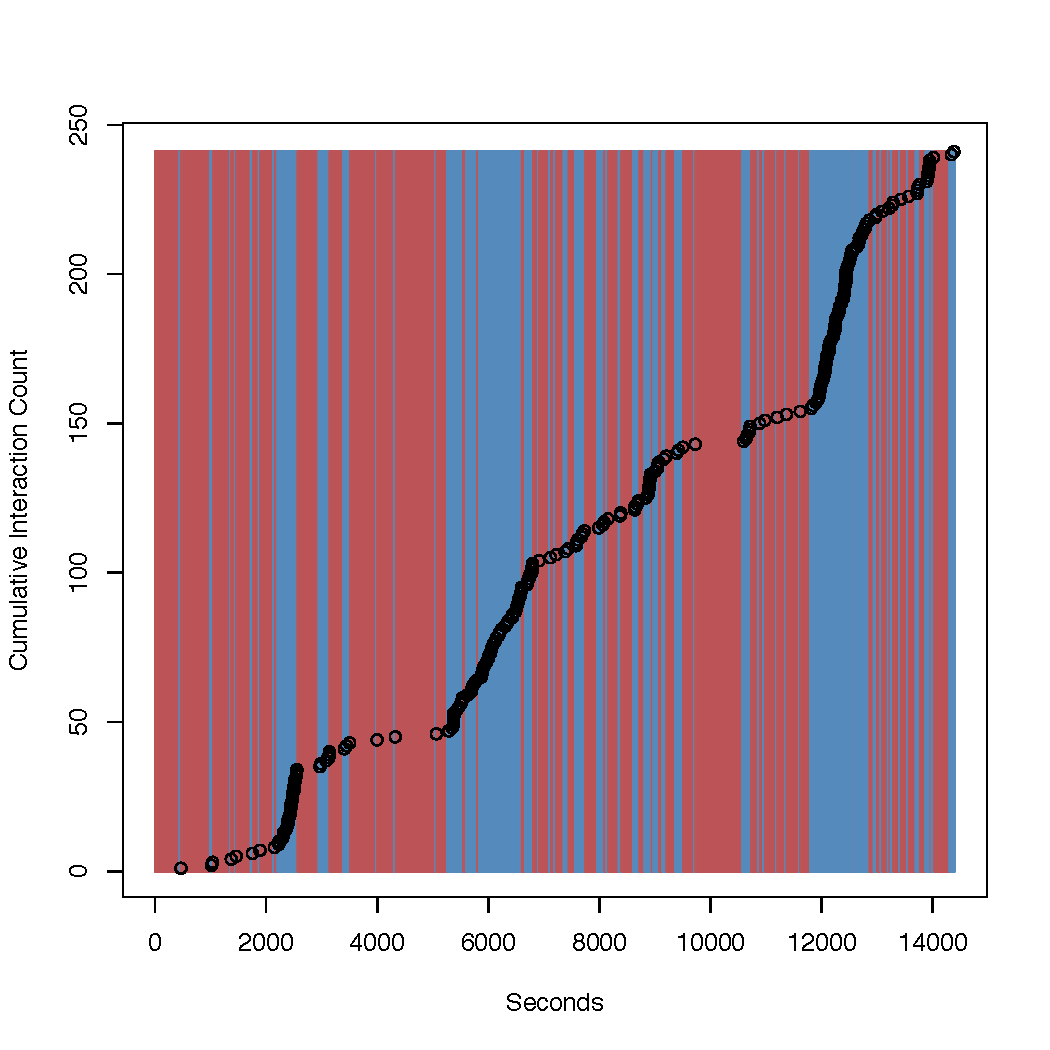
\includegraphics[width=6in]{Sim2_MSPE120000_states.pdf}}
\caption{While periods of relatively low and high rates of feeding interactions are clear, the stochastic process of chamber-level feeding states is switching between the two much faster than biologically feasible. Red background denotes low state while blue background denotes high state of feeding exchanges.}
\label{f:simplestates}
\end{figure}

	An initial examination of the feeding interactions over time (see Figure \ref{f:simplestates}) suggests there may be periodic pulses in the rates of events. These pulses may reflect some latent underlying chamber-level behavioral states that are driving the different trophallaxis rates over time. For example, foraging ants re-entering the nest (as allowed in this experimental setup) may spark a string of trophallaxis events as they seek to distribute nutrients through the colony. Previous research has also shown that ant colonies have been found to exhibit collective activity cycles (\cite{Richardson2017}). However, although we may observe evidence of these cycles, the mechanisms or causes of switching remain uncertain. The combination of high-resolution observations of each ant feeding exchange with these proposed unobserved chamber-level behavioral states lends itself nicely to exploration via a hidden Markov model. Hidden Markov models are often used to model ecological systems because they allow for behaviors to be correlated over time in a way that accounts for shifts in an underlying state process. HMMs have been used recently  to study animal movement behavior (\cite{Langrock2012,McKellar2015, Patterson2017,Towner2016, VandeKerk2015}), general animal behavior (\cite{DeRuiter2016,Langrock2014,Schliehe-Diecks2012}), as well as other applications within population ecology (\cite{Borchers2013,Gimenez2014, Johnson2016, Leos-Barajas2017a}). 
    
    When fitting a two-state Poisson HMM to the ant feeding interaction observations (described below in Section \ref{s:standard}), the estimated state switching rates were much too fast to be biologically reasonable (Figure \ref{f:simplestates}) (switching approximately 0.8 times per minute). In this Figure, the background colors denote the estimated chamber level behavior state. Red background denotes a predicted low state while a blue background denotes the high state of feeding exchanges.  In fact, the best estimated latent chamber level state process often switches between states immediately before and after individual interaction events resulting in fast estimated switching rates. This motivates the need to develop penalized approaches to fitting stochastic processes, like HMMs, to combat the apparent overfitting of the data. High resolution time series are more and more common, so this problem will be important in many future scientific applications. 

    What is typically done in the literature to resolve an issue of short ``state-dwell times'' (i.e. the number of consecutive time points that the Markov chain spends in a given state) is to move to a hidden semi-Markov model (HsMM), which can be expressed in discrete time. While a standard HMM dwell times follow a geometric distribution, Hidden semi-Markov models relax this condition; the dwell time in each state can follow any discrete distribution on the natural numbers (\c CITE YU2009, LANGROCK AND ZUCCINI 2010). However, this approach does not easily allow for the incorportation of covariates. While Langrock and Zucchini propose restructuring HsMM within a specialized HMM design to take advantage of all of the HMM framework. (WHY OURS OVER THIS APPROACH?)

In this paper, we propose a novel penalized hidden Markov model that penalizes rapid state switching through  Bayesian ridge- or LASSO-like priors on continuous-time Markov chain transition rates. We show that this smooths the rate of estimated behavioral state switching and results in better 1-step ahead prediction than the non-penalized HMM. We demonstrate the utility of this penalized approach to stochastic process modeling on the ant trophallaxis data. We then extend this approach to model the effect of biological covariates, such as the arrival of forager ants into the colony or chamber, on transition rates between HMM states in order to better understand the cause of these behavioral switches. 



%% ** The bibliograhy **
\bibliographystyle{ba}
\bibliography{library_20180904}% place <bib-data-file> 

% ** Acknowledgements **
% \begin{acknowledgement}
% \end{acknowledgement}


\end{document}

